\section{Referencia de la Clase Factura\-Proveedor}
\label{classFacturaProveedor}\index{FacturaProveedor@{FacturaProveedor}}
Administra los datos de una factura de proveedor.  


{\tt \#include $<$facturap.h$>$}

Diagrama de herencias de Factura\-Proveedor\begin{figure}[H]
\begin{center}
\leavevmode
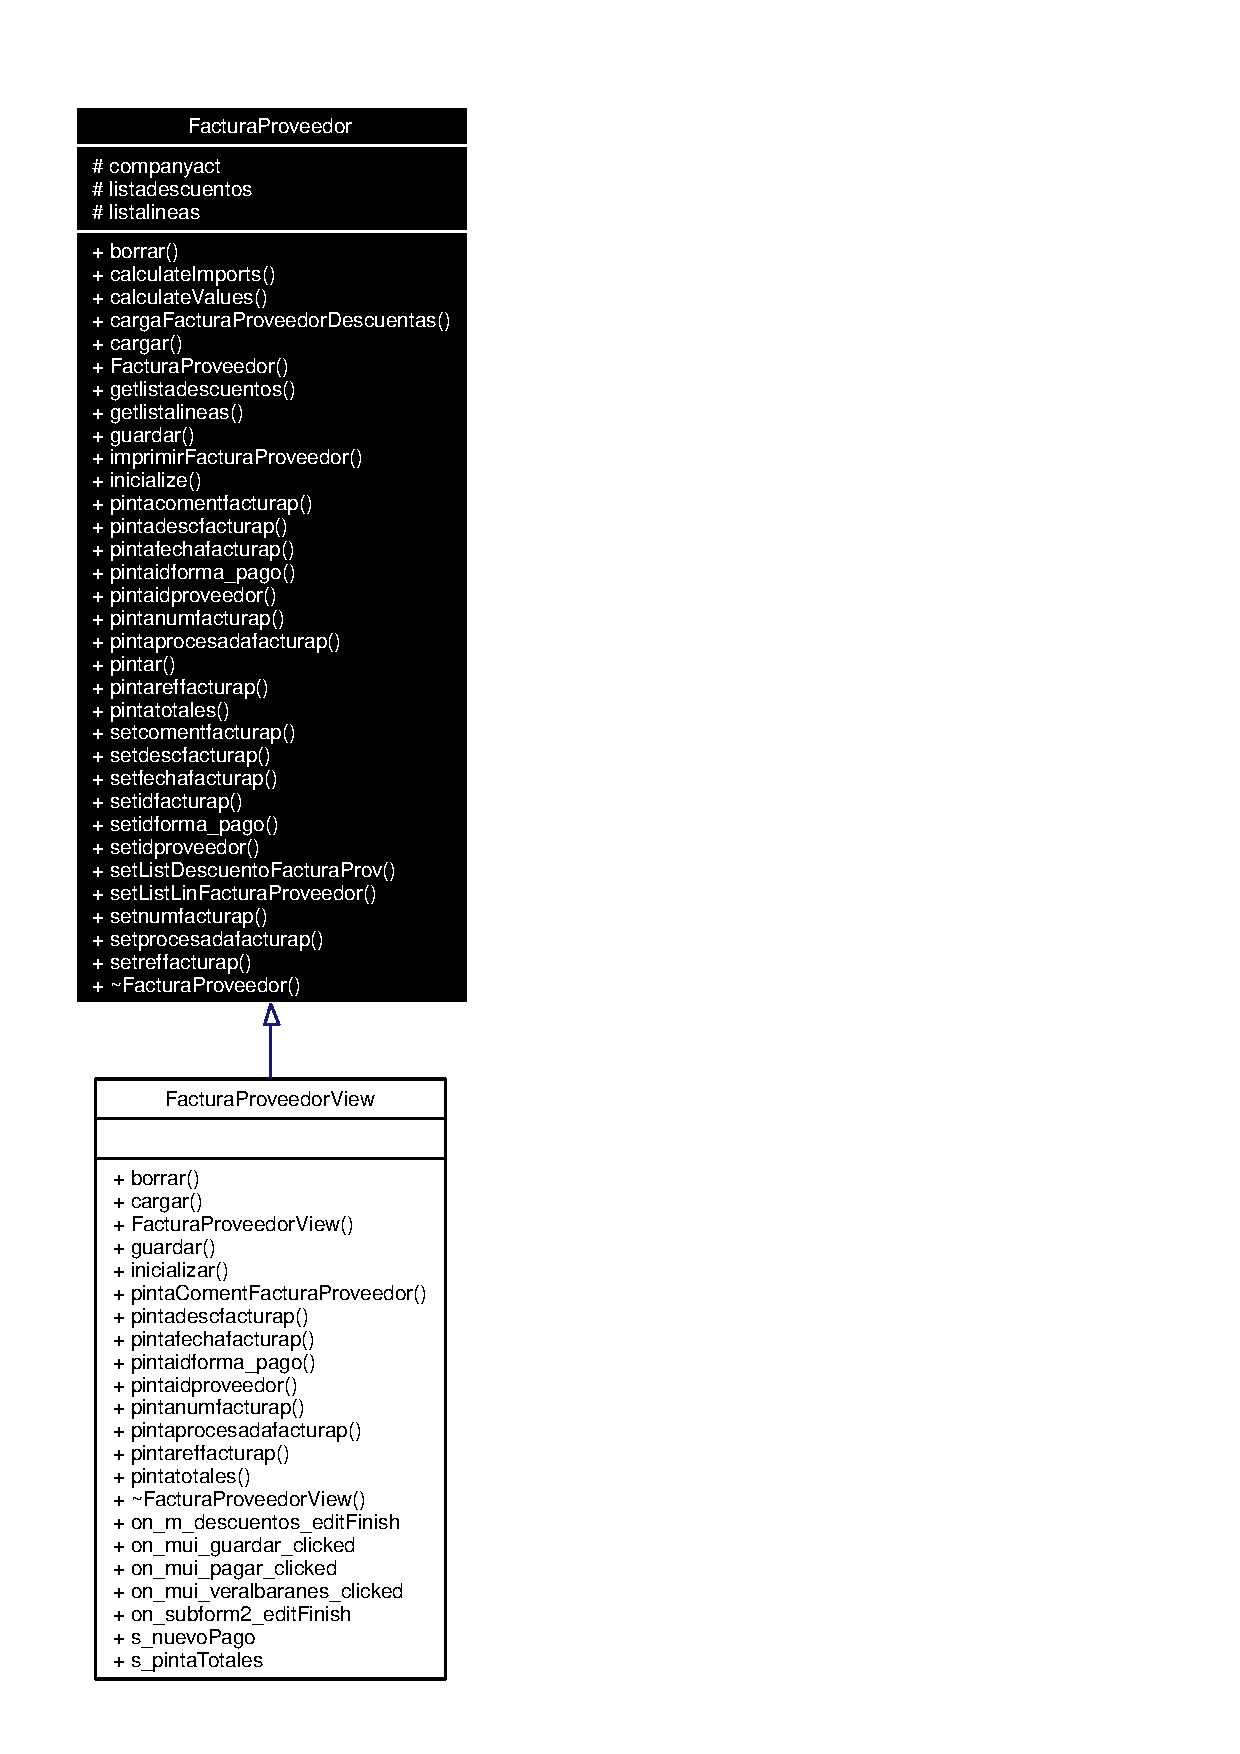
\includegraphics[width=112pt]{classFacturaProveedor__inherit__graph}
\end{center}
\end{figure}
Diagrama de colaboraci\'{o}n para Factura\-Proveedor:\begin{figure}[H]
\begin{center}
\leavevmode
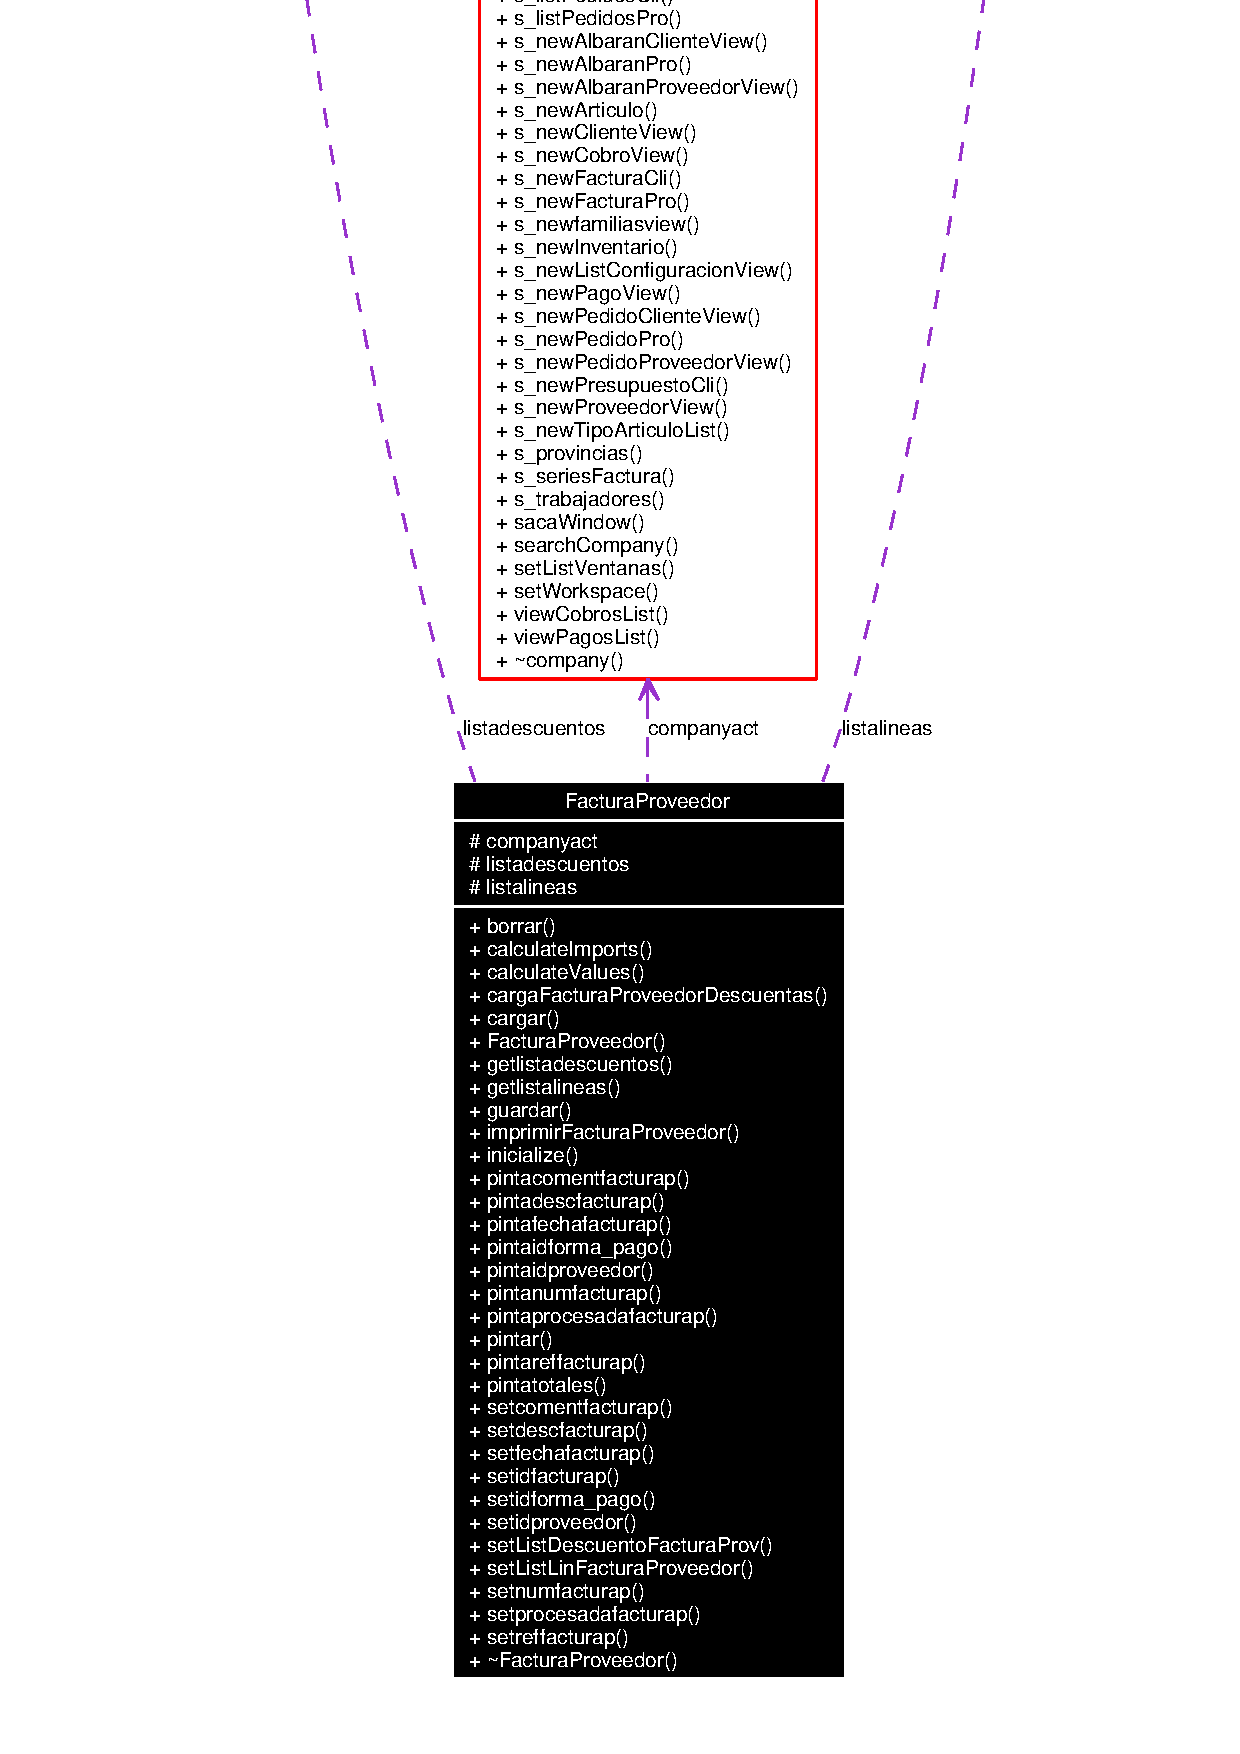
\includegraphics[width=288pt]{classFacturaProveedor__coll__graph}
\end{center}
\end{figure}
\subsection*{M\'{e}todos p\'{u}blicos}
\begin{CompactItemize}
\item 
virtual int {\bf borrar} ()\label{classFacturaProveedor_a0}

\item 
virtual void {\bf calculate\-Imports} ()\label{classFacturaProveedor_a1}

\item 
virtual QString {\bf calculate\-Values} ()\label{classFacturaProveedor_a2}

\item 
virtual void {\bf carga\-Factura\-Proveedor\-Descuentas} (QString)\label{classFacturaProveedor_a3}

\item 
virtual int {\bf cargar} (QString)\label{classFacturaProveedor_a4}

\begin{CompactList}\small\item\em Esta funcion carga un Factura\-Proveedor. \item\end{CompactList}\item 
{\bf Factura\-Proveedor} ({\bf company} $\ast$)\label{classFacturaProveedor_a5}

\item 
{\bf List\-Descuento\-Factura\-Prov\-View} $\ast$ {\bf getlistadescuentos} ()\label{classFacturaProveedor_a6}

\item 
{\bf List\-Lin\-Factura\-Proveedor\-View} $\ast$ {\bf getlistalineas} ()\label{classFacturaProveedor_a7}

\item 
virtual int {\bf guardar} ()\label{classFacturaProveedor_a8}

\item 
virtual void {\bf imprimir\-Factura\-Proveedor} ()
\item 
virtual void {\bf inicialize} ()\label{classFacturaProveedor_a10}

\item 
virtual void {\bf pintacomentfacturap} (QString)\label{classFacturaProveedor_a11}

\item 
virtual void {\bf pintadescfacturap} (QString)\label{classFacturaProveedor_a12}

\item 
virtual void {\bf pintafechafacturap} (QString)\label{classFacturaProveedor_a13}

\item 
virtual void {\bf pintaidforma\_\-pago} (QString)\label{classFacturaProveedor_a14}

\item 
virtual void {\bf pintaidproveedor} (QString)\label{classFacturaProveedor_a15}

\item 
virtual void {\bf pintanumfacturap} (QString)\label{classFacturaProveedor_a16}

\item 
virtual void {\bf pintaprocesadafacturap} (QString)\label{classFacturaProveedor_a17}

\item 
virtual void {\bf pintar} ()\label{classFacturaProveedor_a18}

\item 
virtual void {\bf pintareffacturap} (QString)\label{classFacturaProveedor_a19}

\item 
virtual void {\bf pintatotales} (Fixed, Fixed)\label{classFacturaProveedor_a20}

\item 
void {\bf setcomentfacturap} (QString val)\label{classFacturaProveedor_a21}

\item 
void {\bf setdescfacturap} (QString val)\label{classFacturaProveedor_a22}

\item 
void {\bf setfechafacturap} (QString val)\label{classFacturaProveedor_a23}

\item 
void {\bf setidfacturap} (QString val)\label{classFacturaProveedor_a24}

\item 
void {\bf setidforma\_\-pago} (QString val)\label{classFacturaProveedor_a25}

\item 
void {\bf setidproveedor} (QString val)\label{classFacturaProveedor_a26}

\item 
void {\bf set\-List\-Descuento\-Factura\-Prov} ({\bf List\-Descuento\-Factura\-Prov\-View} $\ast$a)\label{classFacturaProveedor_a27}

\item 
void {\bf set\-List\-Lin\-Factura\-Proveedor} ({\bf List\-Lin\-Factura\-Proveedor\-View} $\ast$a)
\item 
void {\bf setnumfacturap} (QString val)\label{classFacturaProveedor_a29}

\item 
void {\bf setprocesadafacturap} (QString val)\label{classFacturaProveedor_a30}

\item 
void {\bf setreffacturap} (QString val)\label{classFacturaProveedor_a31}

\end{CompactItemize}
\subsection*{Atributos protegidos}
\begin{CompactItemize}
\item 
{\bf company} $\ast$ {\bf companyact}\label{classFacturaProveedor_p0}

\item 
{\bf List\-Descuento\-Factura\-Prov\-View} $\ast$ {\bf listadescuentos}\label{classFacturaProveedor_p1}

\item 
{\bf List\-Lin\-Factura\-Proveedor\-View} $\ast$ {\bf listalineas}\label{classFacturaProveedor_p2}

\end{CompactItemize}


\subsection{Descripci\'{o}n detallada}
Administra los datos de una factura de proveedor. 



\subsection{Documentaci\'{o}n de las funciones miembro}
\index{FacturaProveedor@{Factura\-Proveedor}!imprimirFacturaProveedor@{imprimirFacturaProveedor}}
\index{imprimirFacturaProveedor@{imprimirFacturaProveedor}!FacturaProveedor@{Factura\-Proveedor}}
\subsubsection{\setlength{\rightskip}{0pt plus 5cm}void Factura\-Proveedor::imprimir\-Factura\-Proveedor ()\hspace{0.3cm}{\tt  [virtual]}}\label{classFacturaProveedor_a9}


Hacemos el lanzamiento de plugins para este caso.

Copiamos el archivo.

Copiamos el logo.

Linea de totales del presupuesto

Impresion de la tabla de contenidos.

Contador que sirve para poner lineas de mas en caso de que sea preciso.

Impresion de los descuentos.

Impresion de los totales.

Rellena el primer tr de titulares.

Rellena el segundo tr de cantidades. \index{FacturaProveedor@{Factura\-Proveedor}!setListLinFacturaProveedor@{setListLinFacturaProveedor}}
\index{setListLinFacturaProveedor@{setListLinFacturaProveedor}!FacturaProveedor@{Factura\-Proveedor}}
\subsubsection{\setlength{\rightskip}{0pt plus 5cm}void Factura\-Proveedor::set\-List\-Lin\-Factura\-Proveedor ({\bf List\-Lin\-Factura\-Proveedor\-View} $\ast$ {\em a})\hspace{0.3cm}{\tt  [inline]}}\label{classFacturaProveedor_a28}


Establece cu\'{a}l es la lista subformulario del presupuesto. Normalmente para apuntar listlinpresupuestoview. 

La documentaci\'{o}n para esta clase fu\'{e} generada a partir de los siguientes archivos:\begin{CompactItemize}
\item 
facturap.h\item 
facturap.cpp\end{CompactItemize}
